%----------------------------------------------------------------------------
%----------------------------------------------------------------------------
%				    	SETUP
%----------------------------------------------------------------------------
%----------------------------------------------------------------------------

\documentclass[11pt]{article}

%----------------------------------------------------------------------------
%			  	   PACKAGES
%----------------------------------------------------------------------------

%%%%%%%%%%%%%%%%%%%%%%%
% 	  Packages
%%%%%%%%%%%%%%%%%%%%%%%

%% Fonts and Symbols
%% --------------------------
\usepackage{
	amsmath,			% math operators
	amssymb,			% math symbols
	courier,			% better tt font for listings
	soul,				% strike through with \st{}
	url,				% embed urls in text
	xcolor,				% color!
%	xfrac,				% fancy fractions
}

% preserve default font for URLs
\renewcommand*{\UrlFont}{\rmfamily}		

%% Graphics
%% --------------------
\usepackage{
	graphicx,			% allows insertion of images
	subfigure,			% allows subfigures (a), (b), etc.
}				
\graphicspath{ {graphics/} }	% (graphicx) relative path to graphics folder				

%% Tables
%% --------------------------
\usepackage{
	booktabs,			% better tables, discourages vertical rulings
	multicol,			% allow multi columns
}

%% Layout Alteration
%% --------------------------
\usepackage{			
%	caption,			% line breaks in captions with \\
%	changepage,			% change margins for PARTS of pages with (adjustwidth)
	geometry,			% change the margins for specific PAGES
	parskip,			% disable indents
	rotating,			% sideways figures
	setspace,			% single, double spacing
}
\geometry{				% specify page size options for (geometry)
	a4paper, 			% paper size
	hmargin=1in,		% horizontal margins
	vmargin=1in,		% vertical margins
}	


%% Units
%% --------------------------
\usepackage{
	siunitx,			% has S (decimal align) column type
}
\sisetup{input-symbols = {()},  % do not treat "(" and ")" in any special way
	group-digits  = false, 	% no grouping of digits
%	load-configurations = abbreviations,
%	per-mode = symbol,
}

%% Misc
%% --------------------------
\usepackage{
	enumitem,			% better control of enumerations, descriptions, etc
}

%% References
%% --------------------------
\usepackage[backend=biber,style=ieee]{biblatex}
\addbibresource{ELEC300_Lab_template.bib}

%----------------------------------------------------------------------------
%		     MACROS AND COMMANDS
%----------------------------------------------------------------------------

% Defines a new command for the horizontal lines, change thickness here
\newcommand{\HRule}{\rule{\linewidth}{0.5mm}} 

% override S column type with centered text column
\newcommand{\textcol}[1]{\multicolumn{1}{c}{#1}}


%----------------------------------------------------------------------------
%----------------------------------------------------------------------------
%				   DOCUMENT
%----------------------------------------------------------------------------
%----------------------------------------------------------------------------

\begin{document}

\begin{center}
	\begin{LARGE}
		Department of Electrical and Computer Engineering \\
		University of Victoria \\
		ELEC 300 - Linear Circuits II \\[1cm]
		\textsc{Laboratory Report}
		\\[1cm]
	\end{LARGE}
\end{center}

\begin{tabular}{ p{0.25\textwidth} p{0.75\textwidth} }
	Experiment No.: & 2 \\ 
	Title: & Frequency response of linear systems \\ 
	Date of experiment:& 19 February, 2016 \\ 
	& \\
	Report submitted on:& 26 February, 2016 \\ 
	To: & TA, B07 \\ 
	& \\
	Names: & M. Drinnan (V00755525)\\
	& T. Mulligan (V00819591) \\
	& T. Stephen (V00812021) 
\end{tabular}

\newpage

\doublespacing
\section{Objective}\label{sec:objective}
Short summary of the experiment and results obtained.

\section{Introduction}\label{sec:intro}

\begin{equation}\label{eq:tf}
	H \left( s \right) = K { s - z \over s - p }
\end{equation}

\begin{figure}[tbph]
\centering
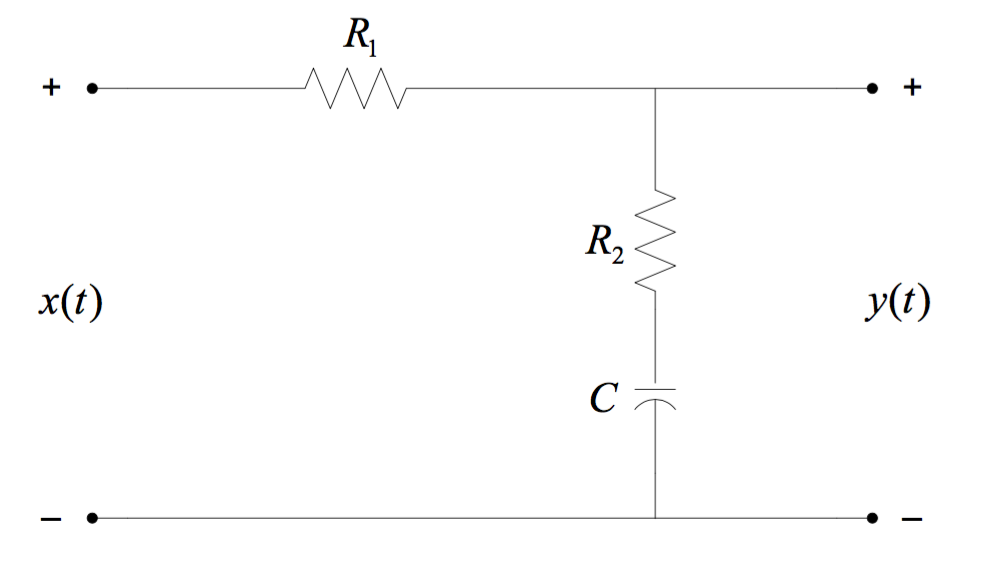
\includegraphics[width=0.7\linewidth]{graphics/lag-schematic}
\caption{Schematic of a phase lag circuit}
\label{fig:schematic}
\end{figure}
For the circuit in Fig. \ref{fig:schematic}, the transfer function is:
\begin{equation}\label{eq:tf-phaselag}
H \left( s \right) = { R_2 + \frac{1}{sC} \over R_1 + R_2 + \frac{1}{sC}} = {R_2 \over R_1 + R_2 } { s + \frac{1}{C R_2} \over s + \frac{1}{C \left( R_1 + R_2 \right)} }.
\end{equation}
Comparing \eqref{eq:tf} with \eqref{eq:tf-phaselag} gives:
\begin{align*}
K &= {R_2 \over R_1 + R_2 } \\
\left|z\right| &= \frac{1}{C R_2} \\
\left|p\right| &= \frac{1}{C \left( R_1 + R_2 \right)}.
\end{align*}

\setkeys{Gin}{width=0.9\textwidth}
\section{Results}\label{sec:results}
Four circuits were assembled and analyzed using a function generator to apply a stimulus, and an oscilloscope to measure the output of the system over the input. A detailed diagram of the circuits which produced these outputs can be referenced in the lab manual \cite{lab-manual}.
\begin{figure}[htbp]
	\centering
	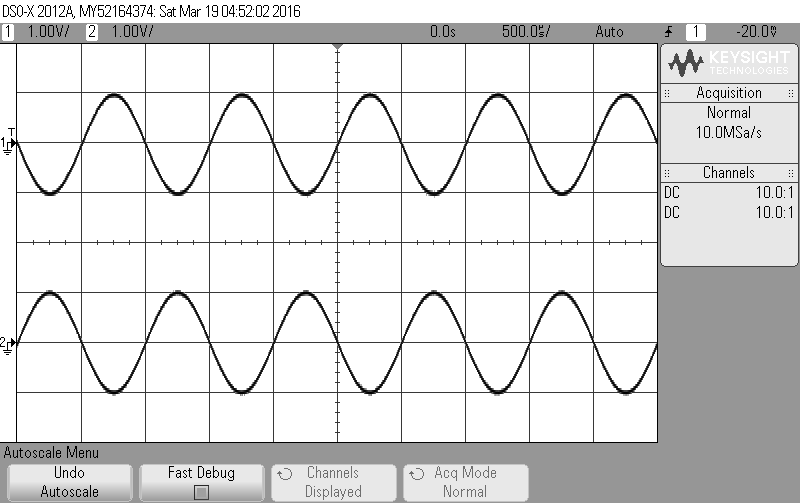
\includegraphics{response-inverter}
	\label{fig:inverter}
	\caption{Input versus output of inverter circuit}
\end{figure}

\begin{figure}[htbp]
	\centering
	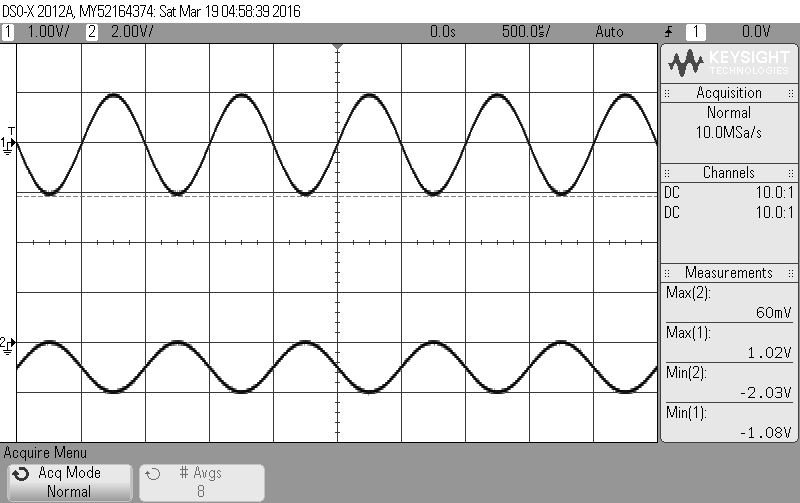
\includegraphics{response-adder}
	\label{fig:adder}
	\caption{Input versus output of adder circuit}
\end{figure}

\begin{figure}[htbp]
	\centering
	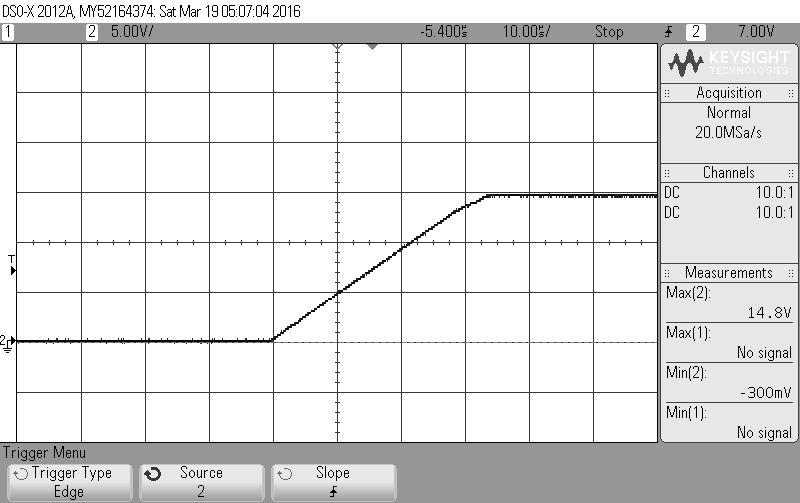
\includegraphics{response-integrator}
	\label{fig:integrator}
	\caption{Input versus output of integrator circuit}
\end{figure}

\begin{figure}
	\centering
	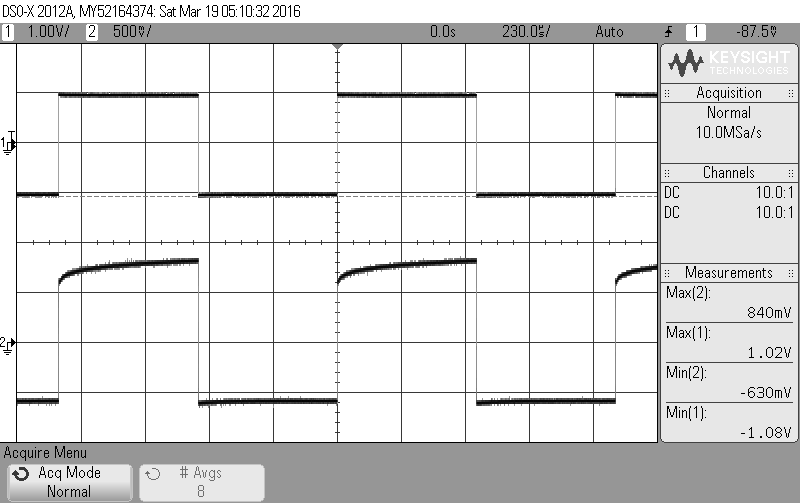
\includegraphics{response-first-order}
	\label{fig:first-order}
	\caption{Input versus output of first order system with an integrator}
\end{figure}

\clearpage

\section{Discussion}\label{sec:discussion}
We confirmed frequency analysis through the Laplace transform is a valid and efficient way to analyze the response of a circuit to inputs of particular or varying frequencies. 

The output of the inverter circuit in Fig.~\ref{fig:inverter} is of equal amplitude to the input waveform, but has a gain of approximately -1. This is the expected behaviour of an inverter circuit.

The adder circuit has an output, visible in Fig.~\ref{fig:inverter} of the same phase as the input signal, however the output signal is the result of adding the input signal to itself, having a gain of 2. This deviates from the experimental procedure of add a DC offset to the input sinusoid, however adding the input to itself confirms the adder circuit functions correctly when both inputs are time varying, or AC signals.

The output of the integrator circuit in Fig.~\ref{fig:integrator} is the result of removing a short across the feedback capacitor, which acts as the integrating element. This ensures the integrator has an initial value of 0, and climbs to the op-amps saturation voltage of 15\si{\volt} when a DC input of approximately -0.1\si{\volt} is provided.

The final circuit, which is a first order system, demonstrates the expected response of such a system to a unit-step input: that is, the system approaches the input signal according to a time-decaying inverse exponential, which is visible in Fig.~\ref{fig:first-order}.

\section{Conclusion}\label{sec:conclusion}
Our results confirm a sinusoid is negatively shifted by a capacitor, as well as the low-pass filter nature of the voltage across a capacitor: when the frequency of the sinusoid across the capacitor the capacitor is low it acts similar to an open circuit, and when the frequency is high the capacitor acts like a short circuit.
The negative phase shift behaviour of a capacitor justifies the circuit's \textit{phase lag} denomination.


\newpage
\printbibliography[heading=bibintoc,title={References}]

\end{document}
